% Options for packages loaded elsewhere
% Options for packages loaded elsewhere
\PassOptionsToPackage{unicode}{hyperref}
\PassOptionsToPackage{hyphens}{url}
\PassOptionsToPackage{dvipsnames,svgnames,x11names}{xcolor}
%
\documentclass[
  english,
  11pt,
  a4paper,
]{article}
\usepackage{xcolor}
\usepackage[top=14mm,bottom=14mm,left=12mm,right=12mm]{geometry}
\usepackage{amsmath,amssymb}
\setcounter{secnumdepth}{-\maxdimen} % remove section numbering
\usepackage{iftex}
\ifPDFTeX
  \usepackage[T1]{fontenc}
  \usepackage[utf8]{inputenc}
  \usepackage{textcomp} % provide euro and other symbols
\else % if luatex or xetex
  \usepackage{unicode-math} % this also loads fontspec
  \defaultfontfeatures{Scale=MatchLowercase}
  \defaultfontfeatures[\rmfamily]{Ligatures=TeX,Scale=1}
\fi
\usepackage{lmodern}
\ifPDFTeX\else
  % xetex/luatex font selection
  \setmainfont[]{Latin Modern Roman}
  \setsansfont[]{Latin Modern Sans}
  \setmonofont[]{Latin Modern Mono}
\fi
% Use upquote if available, for straight quotes in verbatim environments
\IfFileExists{upquote.sty}{\usepackage{upquote}}{}
\IfFileExists{microtype.sty}{% use microtype if available
  \usepackage[]{microtype}
  \UseMicrotypeSet[protrusion]{basicmath} % disable protrusion for tt fonts
}{}
\usepackage{setspace}
\makeatletter
\@ifundefined{KOMAClassName}{% if non-KOMA class
  \IfFileExists{parskip.sty}{%
    \usepackage{parskip}
  }{% else
    \setlength{\parindent}{0pt}
    \setlength{\parskip}{6pt plus 2pt minus 1pt}}
}{% if KOMA class
  \KOMAoptions{parskip=half}}
\makeatother
% Make \paragraph and \subparagraph free-standing
\makeatletter
\ifx\paragraph\undefined\else
  \let\oldparagraph\paragraph
  \renewcommand{\paragraph}{
    \@ifstar
      \xxxParagraphStar
      \xxxParagraphNoStar
  }
  \newcommand{\xxxParagraphStar}[1]{\oldparagraph*{#1}\mbox{}}
  \newcommand{\xxxParagraphNoStar}[1]{\oldparagraph{#1}\mbox{}}
\fi
\ifx\subparagraph\undefined\else
  \let\oldsubparagraph\subparagraph
  \renewcommand{\subparagraph}{
    \@ifstar
      \xxxSubParagraphStar
      \xxxSubParagraphNoStar
  }
  \newcommand{\xxxSubParagraphStar}[1]{\oldsubparagraph*{#1}\mbox{}}
  \newcommand{\xxxSubParagraphNoStar}[1]{\oldsubparagraph{#1}\mbox{}}
\fi
\makeatother


\usepackage{longtable,booktabs,array}
\usepackage{calc} % for calculating minipage widths
% Correct order of tables after \paragraph or \subparagraph
\usepackage{etoolbox}
\makeatletter
\patchcmd\longtable{\par}{\if@noskipsec\mbox{}\fi\par}{}{}
\makeatother
% Allow footnotes in longtable head/foot
\IfFileExists{footnotehyper.sty}{\usepackage{footnotehyper}}{\usepackage{footnote}}
\makesavenoteenv{longtable}
\usepackage{graphicx}
\makeatletter
\newsavebox\pandoc@box
\newcommand*\pandocbounded[1]{% scales image to fit in text height/width
  \sbox\pandoc@box{#1}%
  \Gscale@div\@tempa{\textheight}{\dimexpr\ht\pandoc@box+\dp\pandoc@box\relax}%
  \Gscale@div\@tempb{\linewidth}{\wd\pandoc@box}%
  \ifdim\@tempb\p@<\@tempa\p@\let\@tempa\@tempb\fi% select the smaller of both
  \ifdim\@tempa\p@<\p@\scalebox{\@tempa}{\usebox\pandoc@box}%
  \else\usebox{\pandoc@box}%
  \fi%
}
% Set default figure placement to htbp
\def\fps@figure{htbp}
\makeatother



\ifLuaTeX
\usepackage[bidi=basic]{babel}
\else
\usepackage[bidi=default]{babel}
\fi
\ifPDFTeX
\else
\babelfont{rm}[]{Latin Modern Roman}
\fi
% get rid of language-specific shorthands (see #6817):
\let\LanguageShortHands\languageshorthands
\def\languageshorthands#1{}
\ifLuaTeX
  \usepackage[english]{selnolig} % disable illegal ligatures
\fi


\setlength{\emergencystretch}{3em} % prevent overfull lines

\providecommand{\tightlist}{%
  \setlength{\itemsep}{0pt}\setlength{\parskip}{0pt}}



 


\usepackage{booktabs}
\usepackage{caption}
\usepackage{float}
\usepackage{needspace}
\usepackage{microtype}
\usepackage{fancyhdr}
\captionsetup{font=small,labelfont=bf,labelsep=period,
  justification=raggedright,singlelinecheck=false}
\setlength{\parindent}{0pt}
\setlength{\parskip}{0.45em}
\setlength{\emergencystretch}{2em}
\renewcommand{\arraystretch}{0.9}
\setlength{\tabcolsep}{5pt}
\pagestyle{fancy}
\fancyhf{}
\fancyfoot[C]{\small\thepage}
\setlength{\footskip}{6mm}
\renewcommand{\headrulewidth}{0pt}
\renewcommand{\footrulewidth}{0pt}
\fancypagestyle{plain}{\fancyhf{}\fancyfoot[C]{\small\thepage}
  \renewcommand{\headrulewidth}{0pt}}
\makeatletter
\@ifpackageloaded{caption}{}{\usepackage{caption}}
\AtBeginDocument{%
\ifdefined\contentsname
  \renewcommand*\contentsname{Table of contents}
\else
  \newcommand\contentsname{Table of contents}
\fi
\ifdefined\listfigurename
  \renewcommand*\listfigurename{List of Figures}
\else
  \newcommand\listfigurename{List of Figures}
\fi
\ifdefined\listtablename
  \renewcommand*\listtablename{List of Tables}
\else
  \newcommand\listtablename{List of Tables}
\fi
\ifdefined\figurename
  \renewcommand*\figurename{Figure}
\else
  \newcommand\figurename{Figure}
\fi
\ifdefined\tablename
  \renewcommand*\tablename{Table}
\else
  \newcommand\tablename{Table}
\fi
}
\@ifpackageloaded{float}{}{\usepackage{float}}
\floatstyle{ruled}
\@ifundefined{c@chapter}{\newfloat{codelisting}{h}{lop}}{\newfloat{codelisting}{h}{lop}[chapter]}
\floatname{codelisting}{Listing}
\newcommand*\listoflistings{\listof{codelisting}{List of Listings}}
\makeatother
\makeatletter
\makeatother
\makeatletter
\@ifpackageloaded{caption}{}{\usepackage{caption}}
\@ifpackageloaded{subcaption}{}{\usepackage{subcaption}}
\makeatother
\usepackage{bookmark}
\IfFileExists{xurl.sty}{\usepackage{xurl}}{} % add URL line breaks if available
\urlstyle{same}
\hypersetup{
  pdftitle={MAST32001 Computational Statistics --- Course Assignment},
  pdfauthor={Kaiwei Fu; Lingyu Wang; Sami Pönkä; Zhi Zhou},
  pdflang={en},
  colorlinks=true,
  linkcolor={black},
  filecolor={Maroon},
  citecolor={black},
  urlcolor={black},
  pdfcreator={LaTeX via pandoc}}


\title{MAST32001 Computational Statistics --- Course Assignment}
\author{Kaiwei Fu \and Lingyu Wang \and Sami Pönkä \and Zhi Zhou}
\date{24 October 2026}
\begin{document}
\maketitle


\setstretch{1.05}
\section{Task 1: Ladle Estimation of Signal Dimension Using Time Series
Bootstrap
Methods}\label{task-1-ladle-estimation-of-signal-dimension-using-time-series-bootstrap-methods}

We estimate the signal dimension of a multivariate time series using the
Ladle criterion, which combines lagged dependence with bootstrap
subspace stability. Simulations assess the effects of sample size,
bootstrap method, and block length, followed by an application to the
course dataset.

We use the second-order source separation model

\[
x_t=\mu+\Omega z_t,\qquad E(z_t)=0,\qquad \operatorname{Cov}(z_t)=I_p,
\]

where \(\Omega\) is a nonsingular mixing matrix and \(z_t\) contains
weakly stationary latent components. The first \(q\) components are
mutually independent signals with second-order serial dependence; the
remaining \(p-q\) components are white noise and independent of the
signals. The signal dimension \(q\) is therefore the number of latent
signal components, rather than a count of observed variables. To
identify all \(q\) signals through lagged covariances, the selected lag
set must include at least one lag with nonzero autocovariance for each
signal.

\subsection{Data Preprocessing and Characterization of Lagged
Dependence}\label{data-preprocessing-and-characterization-of-lagged-dependence}

Whitening gives the data an identity sample covariance matrix. Under a
second-order source separation model, it transforms the mixing matrix
into an orthogonal matrix, allowing signal directions to be estimated by
orthogonal joint diagonalization. Lagged dependence remains and provides
the information needed to identify these directions.

\subsubsection{Whitening Transformation and Autocovariance
Estimation}\label{whitening-transformation-and-autocovariance-estimation}

Observations are stored as rows of an \(n\times p\) matrix \(X\). Each
variable is centered using its full-sample column mean:

\[
X_c=X-\mathbf{1}_n\bar{x}^{\mathsf T},
\qquad
S_0=\frac{1}{n-1}X_c^{\mathsf T}X_c.
\]

If \(S_0=VDV^{\mathsf T}\), the symmetric whitening matrix and the
whitened data are

\[
W=S_0^{-1/2}=VD^{-1/2}V^{\mathsf T},
\qquad Y=X_cW.
\]

To avoid unstable inverse square roots, whitening is stopped with an
error if any eigenvalue is at most \(10^{-10}\) times the largest
eigenvalue, indicating a singular or nearly singular covariance matrix.
The whitening matrix already accounts for differences in scale.

For lag \(h\geq1\), we estimate

\[
\widehat C_h
=\frac{1}{n-h}\sum_{t=1}^{n-h}y_ty_{t+h}^{\mathsf T}.
\]

This estimator uses the full-sample means and averages over the \(n-h\)
available pairs of observations separated by lag \(h\). The matrices
used for joint diagonalization are symmetrized as
\(\widehat C_h^{(s)}=(\widehat C_h+\widehat C_h^{\mathsf T})/2\).

\subsubsection{Preprocessing Results and Numerical
Validation}\label{preprocessing-results-and-numerical-validation}

The supplied dataset contains \(n=1000\) observations of \(p=10\)
variables. After centering and whitening,

\[
\max_j|\bar y_j|=6.49\times10^{-14},\qquad
\max_{j,k}\left|\left\{\widehat{\operatorname{Cov}}(Y)-I_{10}\right\}_{jk}\right|
=3.55\times10^{-15}.
\]

The sample means are zero and the sample covariance is the identity up
to numerical precision. Lagged covariances remain nonzero, with
Frobenius norms of \(0.365\) and \(0.558\) at lags 1 and 2.

\begin{figure}[H]

\centering{

\includegraphics[width=0.88\linewidth,height=\textheight,keepaspectratio]{output/figures/task1_whitening_covariance.png}

}

\caption{\label{fig-task1-whitening}Contemporaneous correlation matrix
before whitening (left) and covariance matrix after whitening (right).
Colors indicate matrix entries; the identity pattern on the right
confirms unit variances and negligible cross-covariances.}

\end{figure}%

\subsection{Bootstrap Resampling That Preserves Temporal
Dependence}\label{bootstrap-resampling-that-preserves-temporal-dependence}

Independent row resampling destroys the temporal dependence needed for
signal identification. We instead resample blocks of consecutive
observations, preserving local temporal dependence and keeping all
variables together within each observation.

\subsubsection{Fixed-Block Bootstrap}\label{fixed-block-bootstrap}

Sample \(\lceil n/L\rceil\) starting positions uniformly with
replacement from \(\{1,\ldots,n-L+1\}\). Retain the \(L\) consecutive
observations from each position, concatenate the blocks, and truncate to
\(n\) rows. Dependence is preserved within each block.

\subsubsection{Stationary Bootstrap}\label{stationary-bootstrap}

The stationary bootstrap begins by sampling a starting index uniformly
from \(\{1,\ldots,n\}\). At each subsequent position, a new index is
sampled uniformly with probability \(r=1/L\); otherwise, the previous
index is advanced by one, wrapping from \(n\) back to 1. The block
lengths \(K\) therefore follow a geometric distribution:

\[
\Pr(K=k)=r(1-r)^{k-1},\qquad E(K)=\frac{1}{r}=L.
\]

Conditional on the observed data, the uniform starting index, random
restarts, and circular continuation produce a stationary resampling
process: its joint distributions are invariant to shifts in time. This
property motivates the name stationary bootstrap. Fixed-length block
concatenation generally does not preserve stationarity because block
boundaries occur at predetermined positions.

Across 100 bootstrap samples, the observed mean block lengths were 9.94,
20.20, and 40.94 for target values of 10, 20, and 40, respectively,
close to their intended values.

\subsubsection{Dependence Preservation and Comparison of Block
Lengths}\label{dependence-preservation-and-comparison-of-block-lengths}

We compare preservation of the sample autocorrelation function (ACF),
using independent and identically distributed (IID) resampling as a
reference. Figure~\ref{fig-task1-acf-comparison} shows one
representative variable.

\begin{figure}[H]

\centering{

\includegraphics[width=0.78\linewidth,height=\textheight,keepaspectratio]{output/figures/task1_bootstrap_acf_comparison.png}

}

\caption{\label{fig-task1-acf-comparison}Sample ACFs for the variable
with the largest absolute lag-1 autocorrelation: original data and one
sample from each bootstrap method. Both block methods use \(L=20\); IID
resampling largely removes the lagged dependence.}

\end{figure}%

Dependence preservation is assessed using the mean absolute difference
between the autocorrelations of the original and bootstrap samples,
averaged over all 10 variables and lags 1--20. Each row in
Table~\ref{tbl-task1-acf-error} summarizes 100 bootstrap samples.

\begin{longtable}[]{@{}lrr@{}}
\caption{Mean absolute ACF error; smaller values indicate better
preservation of local
dependence.}\label{tbl-task1-acf-error}\tabularnewline
\toprule\noalign{}
Method & Mean error & Standard deviation \\
\midrule\noalign{}
\endfirsthead
\toprule\noalign{}
Method & Mean error & Standard deviation \\
\midrule\noalign{}
\endhead
\bottomrule\noalign{}
\endlastfoot
IID resampling & 0.0460 & 0.0017 \\
Fixed-block, \(L=10\) & 0.0381 & 0.0021 \\
Fixed-block, \(L=20\) & 0.0320 & 0.0019 \\
Fixed-block, \(L=40\) & 0.0270 & 0.0025 \\
Stationary, \(E(K)=10\) & 0.0336 & 0.0020 \\
Stationary, \(E(K)=20\) & 0.0295 & 0.0024 \\
Stationary, \(E(K)=40\) & 0.0269 & 0.0027 \\
\end{longtable}

IID resampling produces the largest mean error. Longer blocks reproduce
the observed ACF more closely, although the errors are slightly more
variable at \(L=40\). Increasing block length preserves longer stretches
of dependence but reduces the number of blocks resampled.

\begin{figure}[H]

\centering{

\includegraphics[width=0.9\linewidth,height=\textheight,keepaspectratio]{output/figures/task1_bootstrap_acf_error.png}

}

\caption{\label{fig-task1-acf-error}Boxplots of mean absolute ACF error
across 100 bootstrap samples per setting, averaged over 10 variables and
lags 1--20. Lower values indicate better preservation of the original
ACFs.}

\end{figure}%

\subsection{Ladle Estimation Combining Signal Strength and Subspace
Stability}\label{ladle-estimation-combining-signal-strength-and-subspace-stability}

The Ladle criterion combines the strength of lagged dependence with the
stability of estimated subspaces across bootstrap samples.

\subsubsection{\texorpdfstring{Signal Strength and the Scree Component
\(\phi\)}{Signal Strength and the Scree Component \textbackslash phi}}\label{signal-strength-and-the-scree-component-phi}

For a set of lags \(\mathcal T\), an orthogonal matrix \(U\) is used to
approximately jointly diagonalize the autocovariance matrices of the
whitened data. Component strengths are defined as

\[
s_j=\sum_{h\in\mathcal T}
\left[
\operatorname{diag}\!\left(U^{\mathsf T}\widehat C_h^{(s)}U\right)_j
\right]^2,
\]

and ordered as \(s_0\geq\cdots\geq s_{p-1}\). The normalized scree
component is

\[
\phi(k)=\frac{s_k}{1+\sum_{\ell=0}^{p-1}s_\ell},
\qquad k=0,\ldots,p-1.
\]

Larger strengths indicate stronger dependence at the selected lags,
whereas noise directions should have strengths close to zero. For
multiple lags, we obtain \(U\) using \texttt{JADE::rjd}, then compute
and order the component strengths.

\subsubsection{\texorpdfstring{Subspace Instability and the Bootstrap
Component
\(f\)}{Subspace Instability and the Bootstrap Component f}}\label{subspace-instability-and-the-bootstrap-component-f}

Let \(\widehat B_k\) and \(B^*_{k,b}\) contain the first \(k\) ordered
directions from the original sample and the \(b\)th bootstrap sample,
respectively. Subspace instability is measured by

\[
f_0(k)=\frac{1}{B}\sum_{b=1}^{B}
\left\{1-\left|\det\!\left(\widehat B_k^{\mathsf T}B^*_{k,b}\right)\right|\right\},
\quad k=1,\ldots,p-1,
\qquad f_0(0)=0,
\]

and normalized as

\[
f(k)=\frac{f_0(k)}{1+\sum_{\ell=0}^{p-1}f_0(\ell)}.
\]

The absolute determinant measures agreement between the two
\(k\)-dimensional subspaces and is invariant to sign changes in
individual directions. A stable signal subspace has a small \(f(k)\);
including noise directions tends to increase subspace instability.

\subsubsection{Combined Criterion and Dimension
Estimation}\label{combined-criterion-and-dimension-estimation}

The Ladle criterion combines these two sources of information:

\[
g(k)=f(k)+\phi(k),\qquad
\widehat q=\underset{k\in\{0,\ldots,p-1\}}{\arg\min}\;g(k).
\]

As \(k\) increases, the scree component decreases, while the bootstrap
component tends to rise when unstable noise directions enter the
subspace. Minimizing their sum favors a dimension that captures the
signal without including unstable directions.

\subsubsection{Implementation Validation with a Known
Dimension}\label{implementation-validation-with-a-known-dimension}

We check the implementation using Setting 1 of Nordhausen and Virta:
five Gaussian AR/MA signals and five Gaussian white noise series
(\(p=10\), \(q=5\)). With \(n=1000\), lags 1--12, \(B=100\), and
\(L=20\), both bootstrap methods recover \(\widehat q=5\).

Whitening and orthogonality errors are below \(4\times10^{-15}\). After
joint diagonalization, off-diagonal entries account for about \(7.2\%\)
of the squared matrix energy, consistent with approximate rather than
exact diagonalization.

\begin{figure}[H]

\centering{

\includegraphics[width=0.92\linewidth,height=\textheight,keepaspectratio]{output/figures/task1_ladle_criterion.png}

}

\caption{\label{fig-task1-ladle}Ladle curves for one Setting 1 dataset:
bootstrap instability \(f(k)\), scree component \(\phi(k)\), and their
sum \(g(k)\). Both methods minimize \(g(k)\) at the true dimension
\(q=5\) (\(n=1000\), \(B=100\), \(L=20\)).}

\end{figure}%

\subsection{Simulation Study: Signal Dimension
Recovery}\label{simulation-study-signal-dimension-recovery}

\subsubsection{Data-Generating Model and Experimental
Design}\label{data-generating-model-and-experimental-design}

We use Setting 1 of Nordhausen and Virta, with \(p=10\) components and a
true signal dimension of \(q=5\). The mixing matrix is the identity, so
\(x_t=z_t\), where the first five components are mutually independent
Gaussian AR/MA processes and the remaining five are mutually independent
Gaussian white noise series. The signal parameters are listed in
Table~\ref{tbl-de-processes}, using the following convention:

\[
z_{j,t}=\sum_{\ell=1}^{r_j}a_{j,\ell}z_{j,t-\ell}
      +\varepsilon_{j,t}
      +\sum_{\ell=1}^{s_j}b_{j,\ell}\varepsilon_{j,t-\ell},
\qquad \varepsilon_{j,t}\overset{\mathrm{iid}}{\sim}N(0,1).
\]

Innovations are independent across components, and the five noise series
are independent \(N(0,1)\) white noise. Each data column is centered and
scaled to unit sample variance before whitening, as in the
implementation check.

\begin{longtable}[]{@{}cll@{}}
\caption{Signal processes in Setting 1. A dash indicates the absence of
the corresponding AR or MA part.}\label{tbl-de-processes}\tabularnewline
\toprule\noalign{}
Component & AR coefficients & MA coefficients \\
\midrule\noalign{}
\endfirsthead
\toprule\noalign{}
Component & AR coefficients & MA coefficients \\
\midrule\noalign{}
\endhead
\bottomrule\noalign{}
\endlastfoot
1 & \((0.6)\) & \((0,-0.4)\) \\
2 & \((0.4,0.1,0.3)\) & \((0.2,0.4)\) \\
3 & \((0.4)\) & -- \\
4 & -- & \((0.5,0.3,0.1,0.2)\) \\
5 & \((0.1,0.1,0.3)\) & -- \\
\end{longtable}

We use \(n\in\{200,500,1000\}\), SOBI lags
\(\mathcal T=\{1,\ldots,12\}\), and both bootstrap methods with
\(L\in\{10,20,40\}\) (fixed or expected block length). These settings
match the paper; its separate AMUSE comparison is outside our scope.

For each sample size, we generate \(R=100\) independent datasets and
apply all six method--block length combinations, giving \(1800\) fits
with \(B=100\) bootstrap samples each. This is smaller than the paper's
\(R=2000\), \(B=200\) experiment and targets its qualitative findings at
lower computational cost. Here, \(R\) controls the precision of recovery
rates across datasets; \(B\) controls the Monte Carlo approximation
within each fit.

\subsubsection{Computational Procedure and Choice of Tuning
Parameters}\label{computational-procedure-and-choice-of-tuning-parameters}

For each dataset, we apply the following steps.

\begin{enumerate}
\def\labelenumi{\arabic{enumi}.}
\tightlist
\item
  Center and whiten the data, then compute symmetrized autocovariances
  at lags 1--12.
\item
  Jointly diagonalize them using \texttt{JADE::rjd}, order directions by
  their strengths, and compute \(\phi(k)\).
\item
  Generate \(B\) multivariate bootstrap samples using fixed blocks or
  the stationary bootstrap of Politis and Romano. Repeat centering,
  whitening, autocovariance estimation, diagonalization, and ordering
  for each sample.
\item
  Compare the leading subspaces to compute \(f(k)\), then record the
  dimension minimizing \(g(k)=f(k)+\phi(k)\) over \(k=0,\ldots,9\).
\end{enumerate}

Short blocks break more lagged observation pairs: a fixed block of
length \(10\) cannot contain a lag-\(12\) pair. Longer blocks preserve
more dependence but leave fewer blocks to resample; for \(n=200\) and
\(L=40\), only five fixed blocks are drawn.

Data generation and bootstrap fitting use separate random seeds. Shared
datasets allow paired comparisons across settings. After some
preliminary runs reached the \(1000\)-iteration limit, we increased it
to \(10000\), keeping the joint diagonalization tolerance at
\(10^{-6}\). All \(1800\) fits completed, with whitening and
orthogonality errors below \(3\times10^{-14}\) and \(9\times10^{-15}\),
respectively.

\subsubsection{Evaluation Metrics and Monte Carlo
Error}\label{evaluation-metrics-and-monte-carlo-error}

For a fixed sample size, method, and block length, let
\(I_r=\mathbf 1\{\widehat q_r=5\}\). The estimated probability of
correct selection and its Monte Carlo standard error are

\[
\widehat P=\frac{1}{R}\sum_{r=1}^{R}I_r,
\qquad
\widehat{\operatorname{MCSE}}(\widehat P)
=\sqrt{\frac{\widehat P(1-\widehat P)}{R}}.
\]

With \(R=100\), the MCSE is at most \(0.05\). We report \(95\%\) Wilson
intervals, including at observed rates of \(0\) or \(1\), and dimension
distributions to distinguish underestimation from overestimation.

\subsubsection{Effect of Sample Size on Dimension
Recovery}\label{effect-of-sample-size-on-dimension-recovery}

\begin{longtable}[]{@{}lrrrr@{}}
\caption{Percentage of replications selecting the true dimension
\(q=5\). Each value is based on \(100\) independent datasets, with
\(B=100\) bootstrap samples per
fit.}\label{tbl-de-recovery}\tabularnewline
\toprule\noalign{}
Method & \(L\) & \(n=200\) & \(n=500\) & \(n=1000\) \\
\midrule\noalign{}
\endfirsthead
\toprule\noalign{}
Method & \(L\) & \(n=200\) & \(n=500\) & \(n=1000\) \\
\midrule\noalign{}
\endhead
\bottomrule\noalign{}
\endlastfoot
Fixed-block & 10 & 0 & 36 & 99 \\
Fixed-block & 20 & 0 & 37 & 99 \\
Fixed-block & 40 & 1 & 38 & 99 \\
Stationary & 10 & 0 & 34 & 99 \\
Stationary & 20 & 1 & 40 & 99 \\
Stationary & 40 & 1 & 45 & 99 \\
\end{longtable}

Table~\ref{tbl-de-recovery} and Figure~\ref{fig-de-recovery} show that
sample size has the most pronounced effect. When \(n=200\), only
\(0\)--\(1\%\) of replications select the correct dimension. Both
underestimation and overestimation are common, occurring in
\(58\)--\(77\%\) and \(22\)--\(42\%\) of replications, respectively.
When \(n=500\), recovery rates increase to \(34\)--\(45\%\), with most
remaining errors due to underestimation. When \(n=1000\), every setting
selects \(q=5\) in \(99\) replications and \(q=4\) in one replication.
The corresponding \(95\%\) Wilson interval is \([94.6\%,99.8\%]\),
consistent with a high recovery rate at this sample size.

\begin{figure}[H]

\centering{

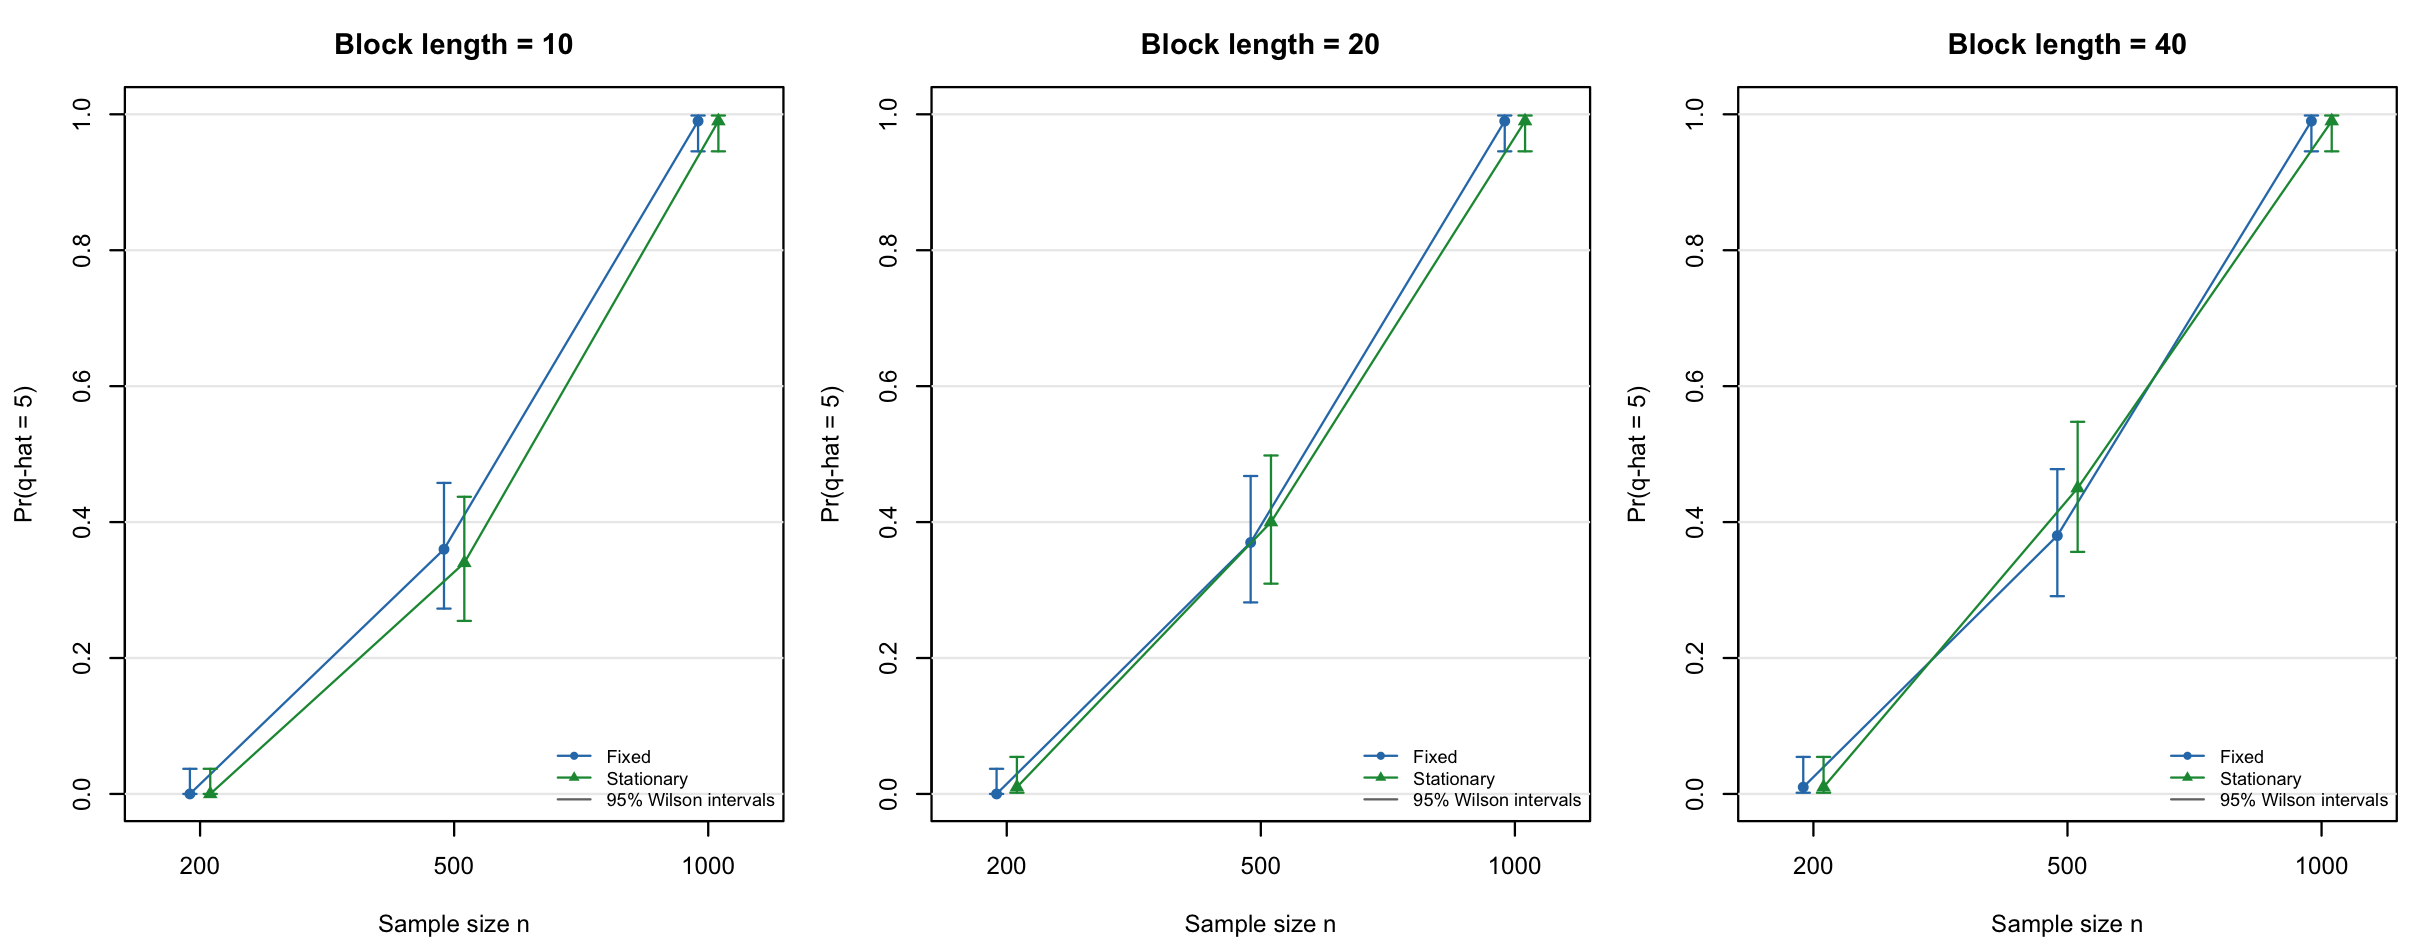
\includegraphics[width=1\linewidth,height=\textheight,keepaspectratio]{output/figures/task1_d_recovery_probability.png}

}

\caption{\label{fig-de-recovery}Estimated probability of selecting
\(q=5\) from 100 simulated datasets per sample size. Panels correspond
to block lengths; blue circles and green triangles denote fixed-block
and stationary bootstrap results. Error bars are \(95\%\) Wilson
intervals.}

\end{figure}%

\subsubsection{Bootstrap Method, Block Length, and the Distribution of
Estimation
Errors}\label{bootstrap-method-block-length-and-the-distribution-of-estimation-errors}

Method differences are smaller than sample-size effects. At \(n=500\),
stationary minus fixed-block recovery rates are \(-2\), \(3\), and \(7\)
percentage points for \(L=10,20,40\), with paired MCSEs of \(3.5\),
\(3.3\), and \(3.8\) points. The MCSEs use within-dataset differences
\(I_{r,S}-I_{r,F}\) to account for pairing. These results do not
establish a clear advantage for either method; at \(n=1000\), all
settings give identical selections.

\begin{figure}[H]

\centering{

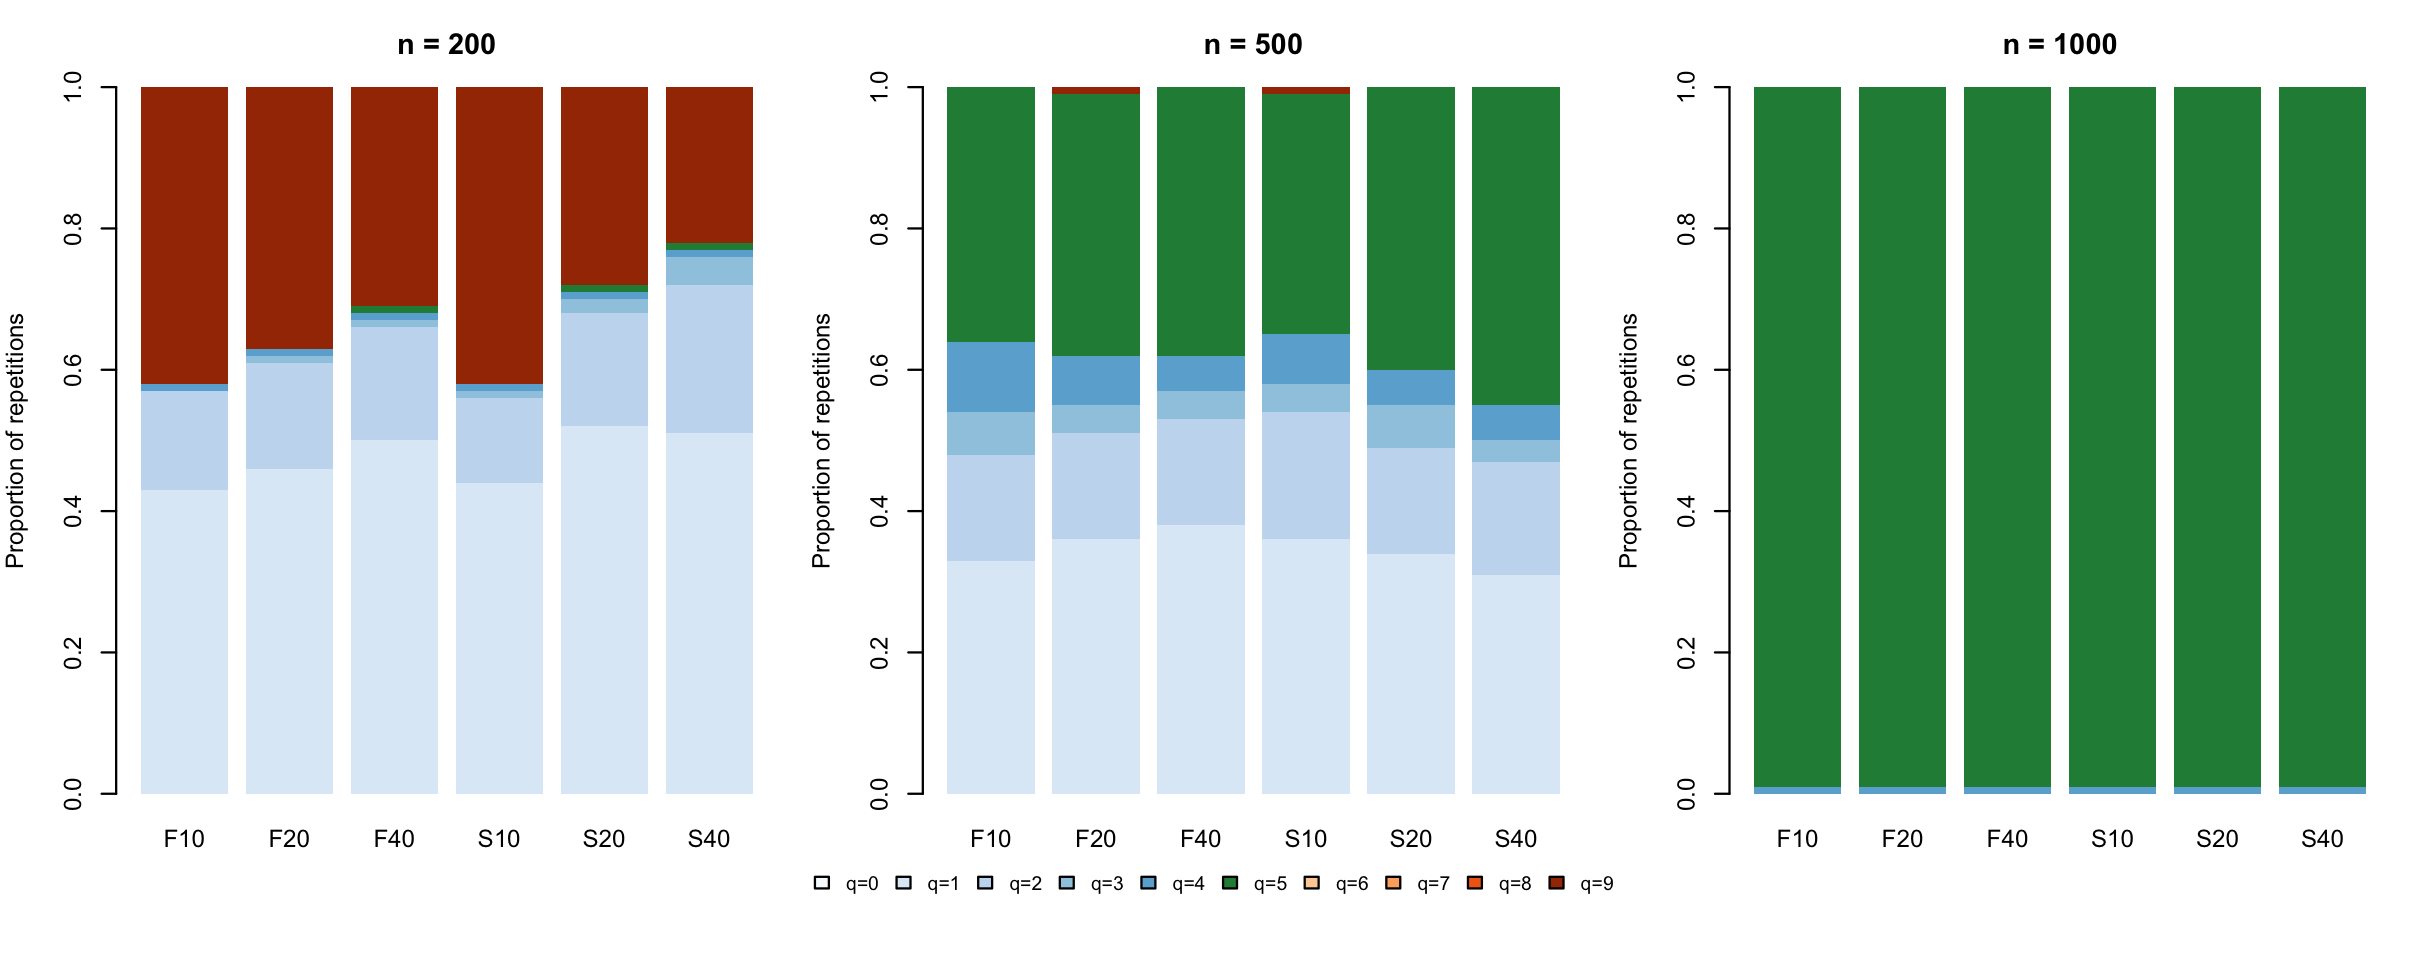
\includegraphics[width=0.95\linewidth,height=\textheight,keepaspectratio]{output/figures/task1_d_dimension_distribution.png}

}

\caption{\label{fig-de-distribution}Stacked proportions of estimated
dimensions across 100 Setting 1 datasets per sample size. F and S denote
fixed-block and stationary bootstrap methods; numbers indicate \(L\).
Green represents the true dimension \(q=5\).}

\end{figure}%

The distributions in Figure~\ref{fig-de-distribution} narrow around
\(q=5\) as series length increases, consistent with Nordhausen and
Virta's qualitative findings. This evidence is limited to Setting 1 with
\(B=100\); it does not establish consistency or reproduce the full
study.

\subsection{Analysis of the Course Dataset: Dimension Estimation and
Sensitivity to Block
Length}\label{analysis-of-the-course-dataset-dimension-estimation-and-sensitivity-to-block-length}

\subsubsection{Analysis Settings and Stability
Assessment}\label{analysis-settings-and-stability-assessment}

We analyze \texttt{timeseries.dat} (\(n=1000\), \(p=10\)) using the same
preprocessing, lags 1--12, and Ladle procedure as in the simulations.
Both bootstrap methods use \(L=10,20,40\). The primary choice, \(L=20\),
accommodates all selected lags within a block and yields \(50\) fixed
blocks; \(L=10\) and \(40\) assess block-length sensitivity.

Each setting uses \(B=500\) bootstrap samples and five independent
random seeds. The resulting \(30\) fits assess Monte Carlo stability for
this dataset, not sampling uncertainty. We examine the criterion curves,
selected dimensions, and gaps between the two lowest values of \(g\).

\subsubsection{Results Supporting a Three-Dimensional Signal
Subspace}\label{results-supporting-a-three-dimensional-signal-subspace}

At \(L=20\) and \(40\), both methods select \(\widehat q=3\) in all five
runs. At \(L=10\), fixed blocks always select \(2\), while stationary
blocks select \(2\) four times and \(3\) once. The latter setting has a
minimum criterion gap of about \(0.0007\), indicating a near tie in at
least one run. Thus, the three-dimensional estimate is stable with
longer blocks but sensitive to short blocks.

For the primary fixed-block fit with \(L=20\) and the first seed,

\[
f(3)=0.04660,\qquad \phi(3)=0.01649,\qquad g(3)=0.06310.
\]

The next-best candidate is \(k=2\), whose criterion value exceeds the
minimum by \(0.01278\). The first four ordered component strengths are
approximately \(0.400\), \(0.345\), \(0.141\), and \(0.034\). The drop
after the third direction supports a three-dimensional signal subspace,
while the bootstrap term penalizes the instability introduced by
additional weak directions.

\begin{figure}[H]

\centering{

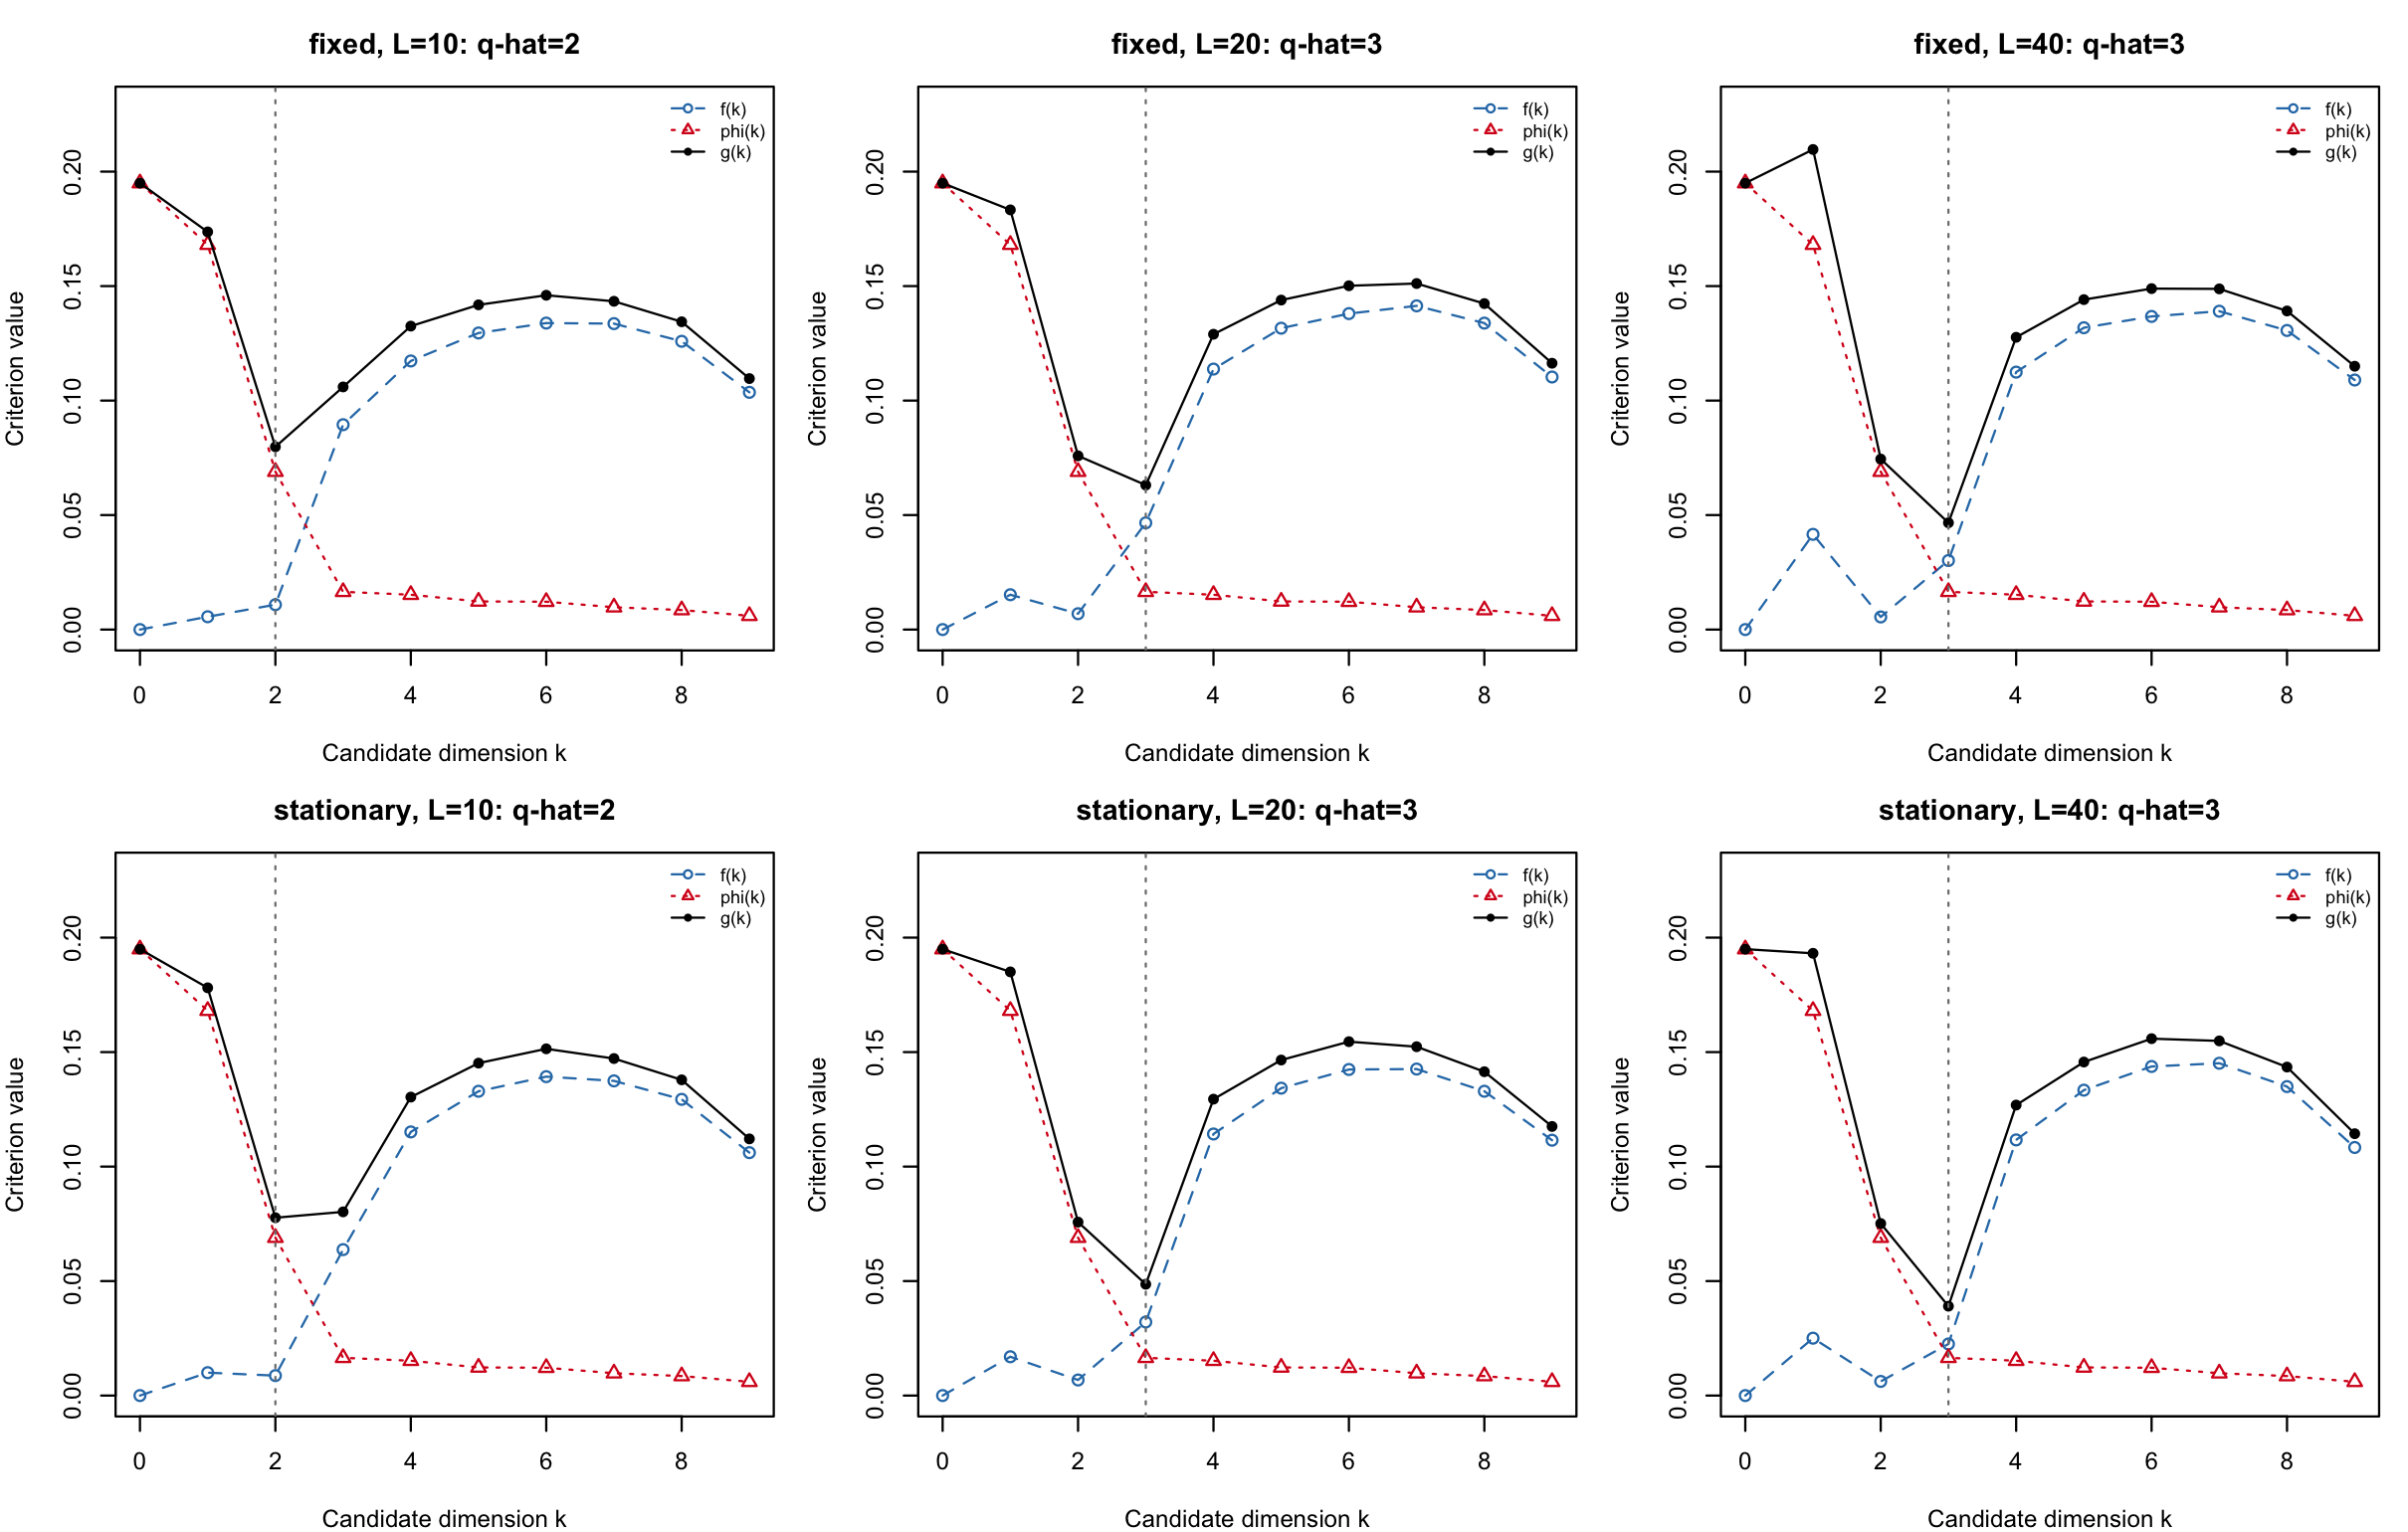
\includegraphics[width=1\linewidth,height=\textheight,keepaspectratio]{output/figures/task1_e_ladle_components.png}

}

\caption{\label{fig-de-components}Ladle components under the six
settings for the course dataset, using the first seed for each setting.
Vertical lines indicate the dimensions minimizing the criterion. Under
the definition above, \(\phi(k)\) corresponds to the strength of the
\((k+1)\)th direction.}

\end{figure}%

In Figure~\ref{fig-de-components}, \(\phi\) depends only on the original
sample and is unchanged across settings. Differences in selection arise
from the bootstrap component \(f\).

\subsubsection{Sensitivity to Block Length and Its Explanation Through
Dependence
Structure}\label{sensitivity-to-block-length-and-its-explanation-through-dependence-structure}

\begin{figure}[H]

\centering{

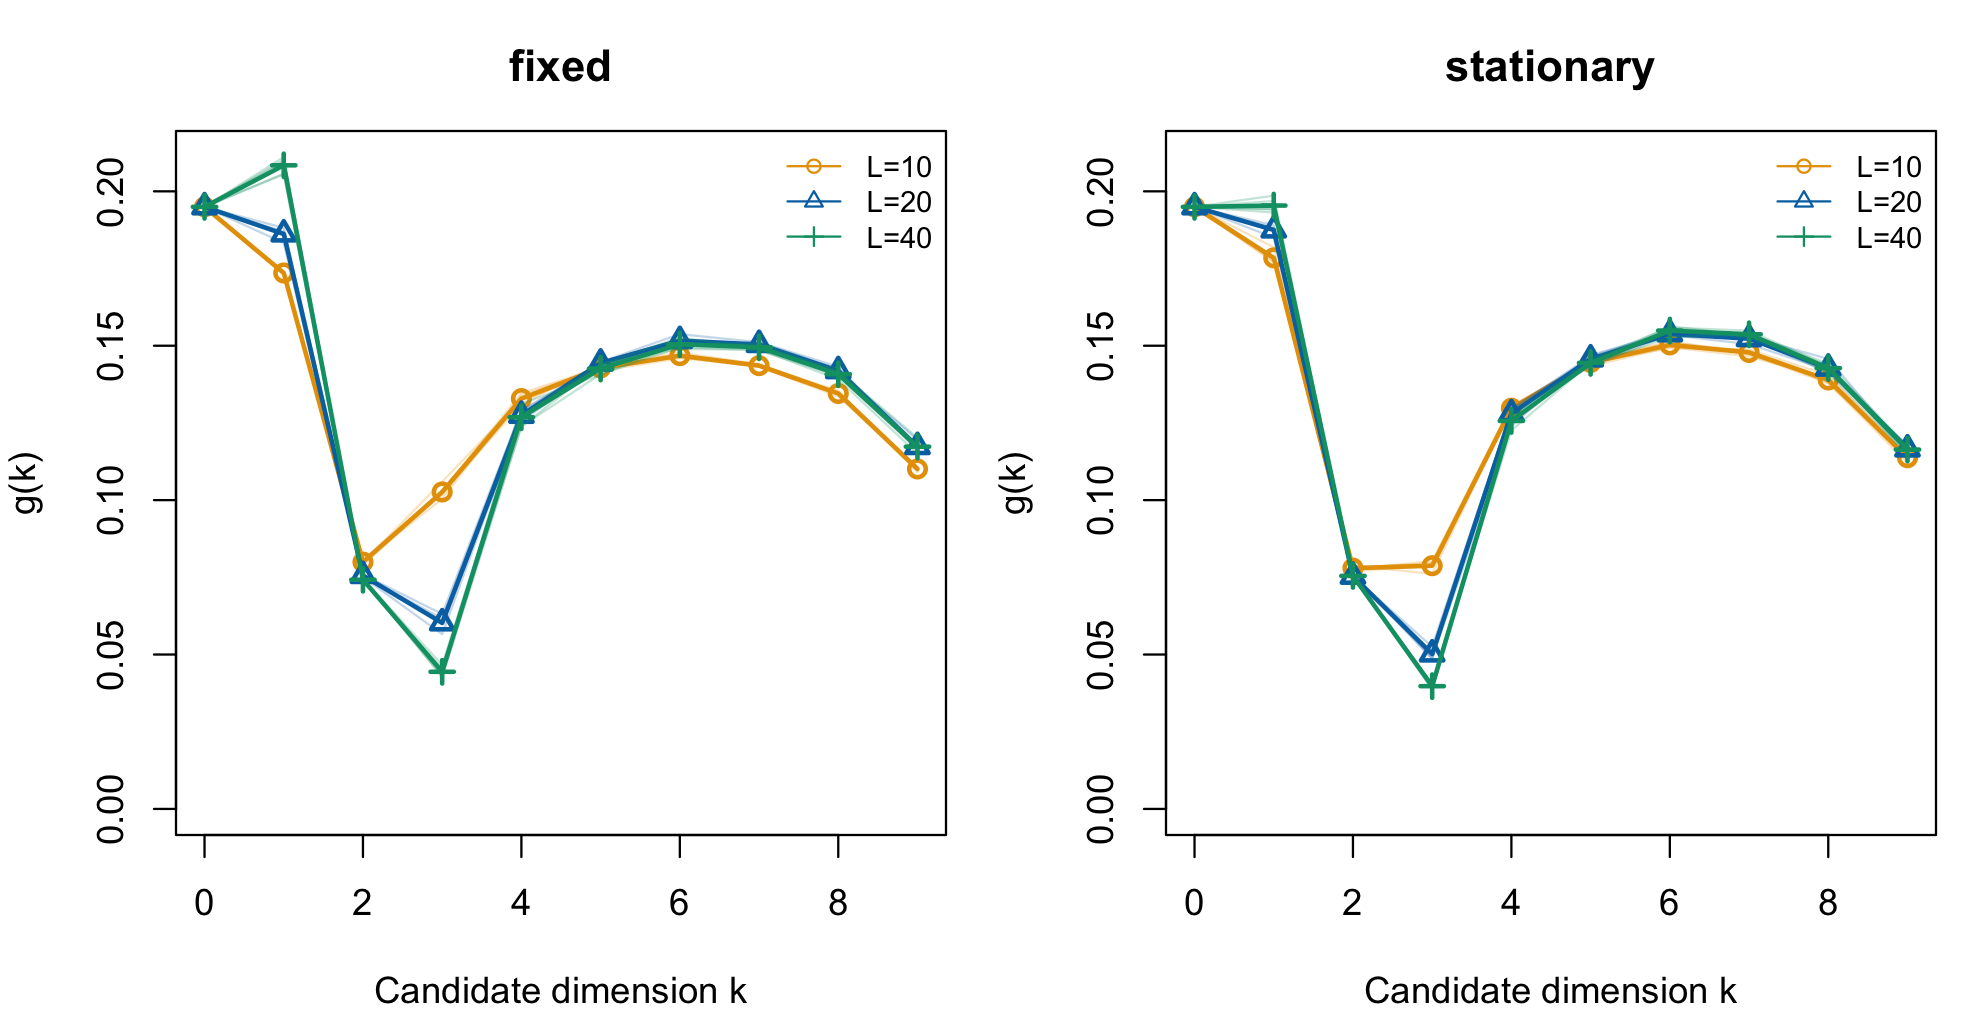
\includegraphics[width=1\linewidth,height=\textheight,keepaspectratio]{output/figures/task1_e_block_sensitivity.png}

}

\caption{\label{fig-de-sensitivity}Total criterion \(g(k)\) by block
length for fixed-block (left) and stationary (right) bootstrap. Colors
distinguish \(L=10,20,40\); light curves show five individual seed runs
and thick curves their means. Dimensions are selected separately for
each run.}

\end{figure}%

To explain the competition between \(k=2\) and \(3\) in
Figure~\ref{fig-de-sensitivity}, we examine the ordered components

\[
\widehat Z=(X-\mathbf 1_n\bar x^{\mathsf T})\widehat W\widehat U.
\]

For the third component, the largest absolute sample autocorrelation
over lags \(1\)--\(12\) occurs at \(h=8\), where the autocorrelation is
approximately \(0.287\). Dependence at this lag may be poorly preserved
by short blocks.

For fixed blocks, ignoring endpoint effects in a finite series, the
proportion of lag-\(h\) observation pairs lying within the same block is
approximately \(\max(1-h/L,0)\). For stationary blocks, the probability
of proceeding for \(h\) consecutive steps without restarting is
\((1-1/L)^h\). At \(h=8\), these quantities are

\[
\begin{array}{c|ccc}
L & 10 & 20 & 40 \\ \hline
\text{Fixed-block: within-block pair proportion} & 0.200 & 0.600 & 0.800 \\
\text{Stationary: probability of no restart} & 0.430 & 0.663 & 0.817
\end{array}
\]

These are measures of preserved ordering, not exact ACF attenuation
factors or recovery probabilities. They suggest that short blocks weaken
the dependence supporting the third direction, making its estimated
subspace less stable. The more distinct minimum at \(k=3\) with longer
blocks is consistent with this explanation.

\begin{figure}[H]

\centering{

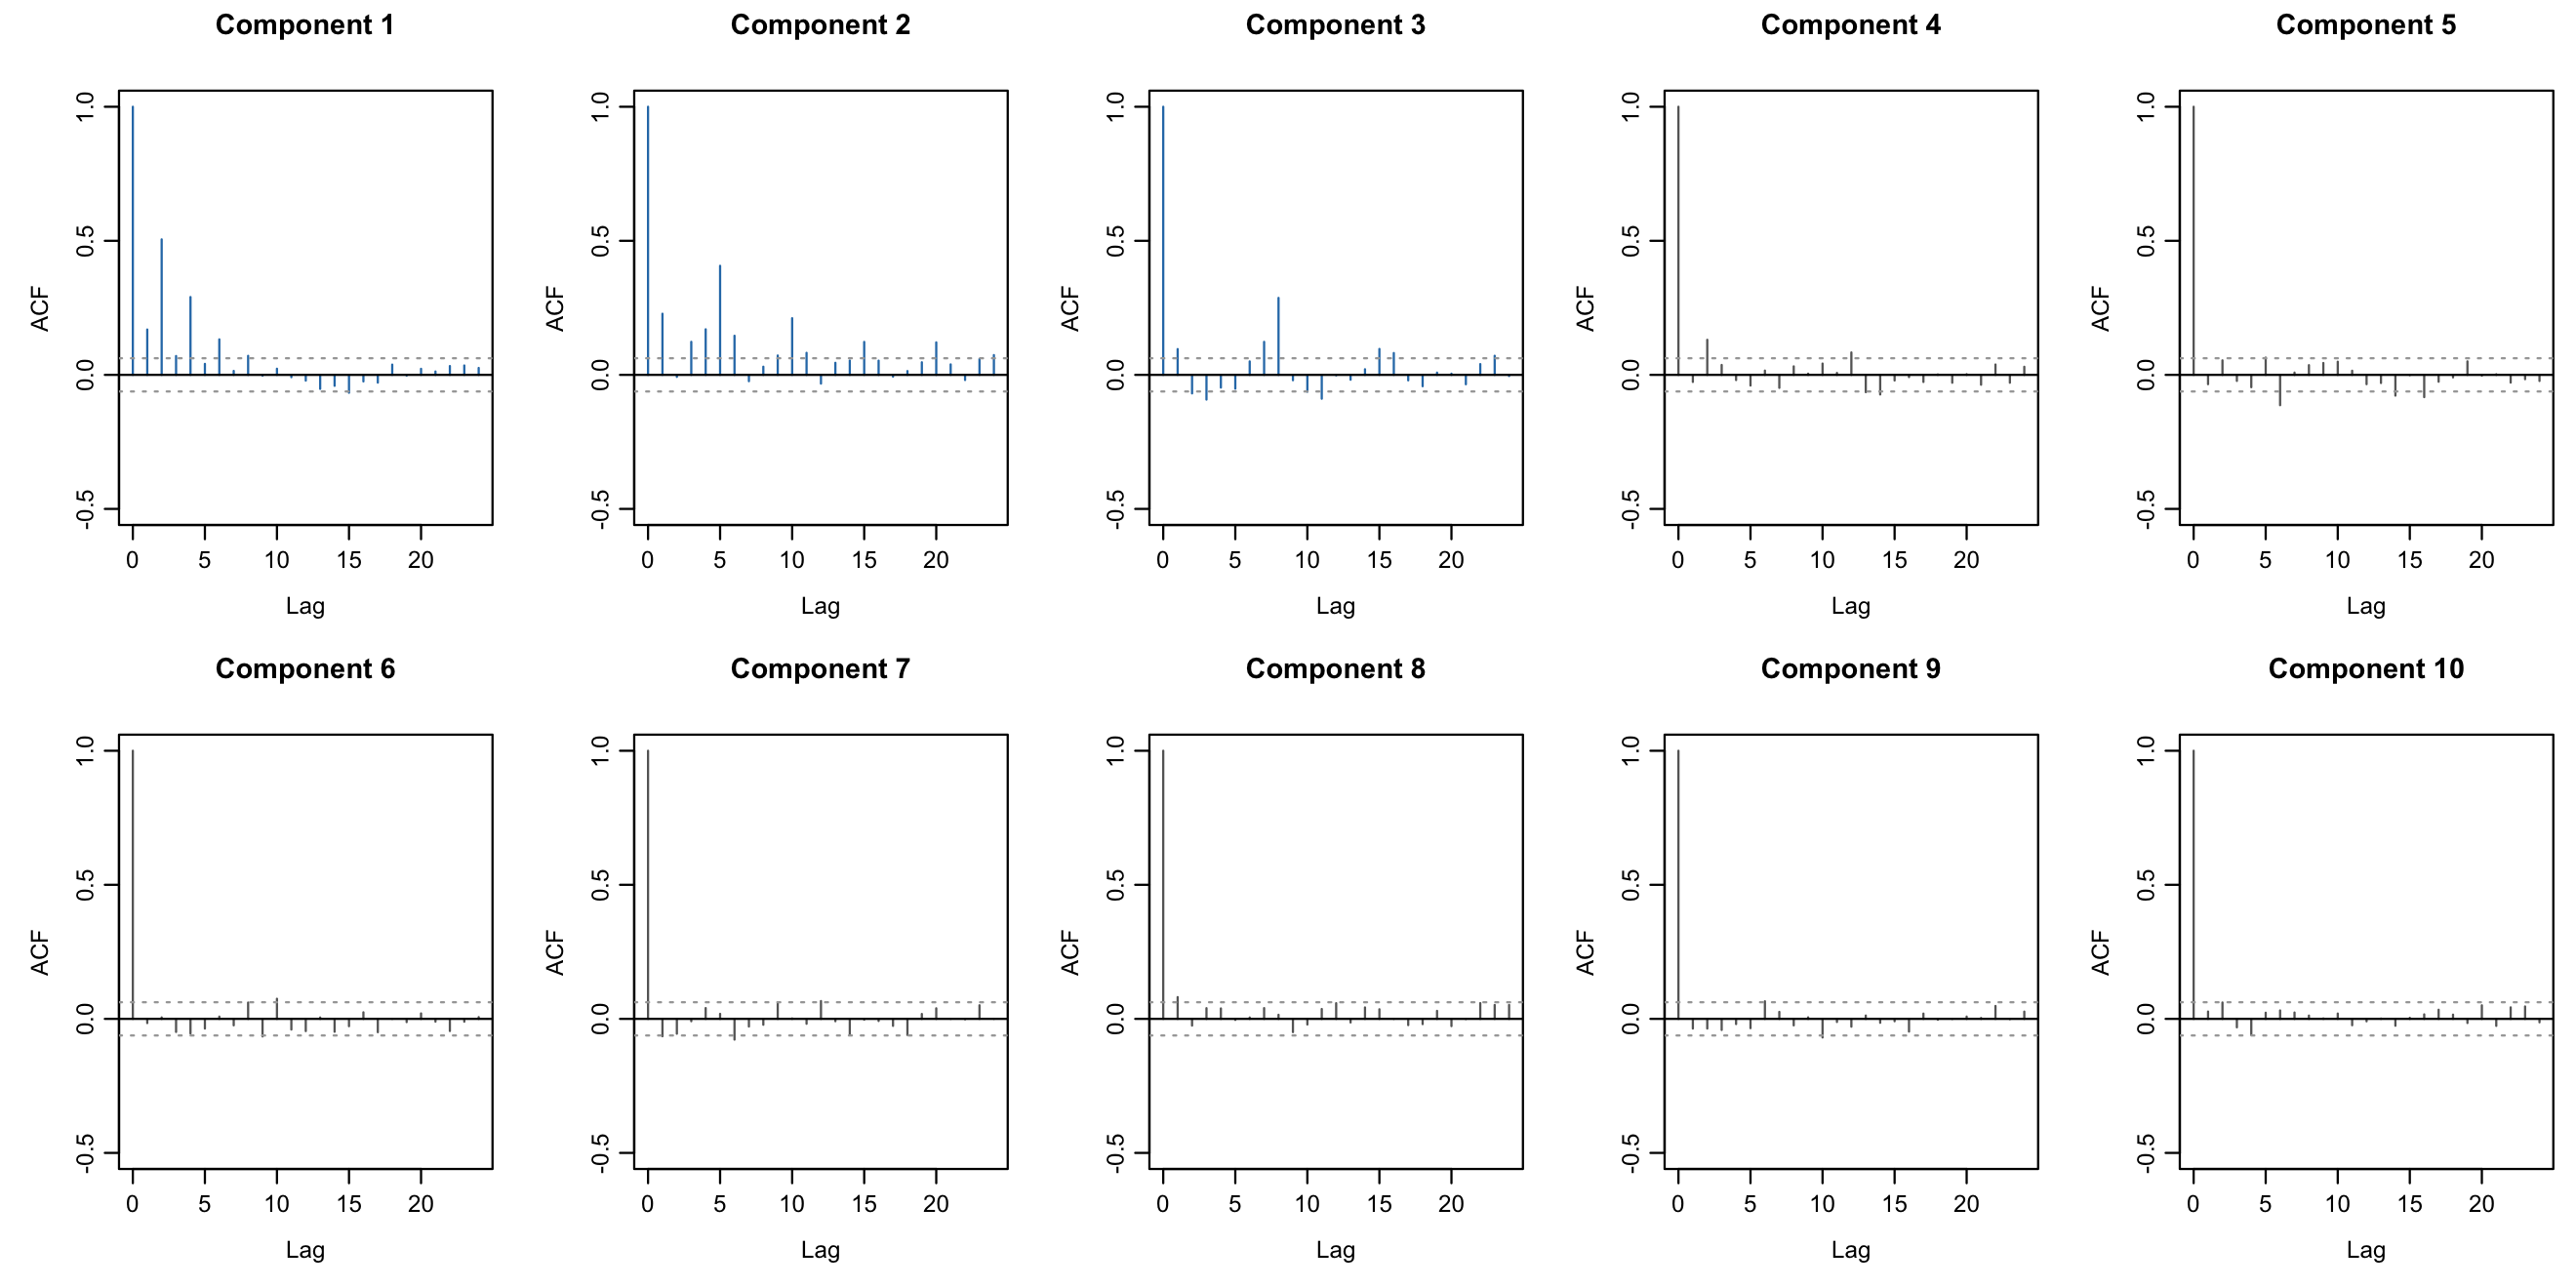
\includegraphics[width=1\linewidth,height=\textheight,keepaspectratio]{output/figures/task1_e_component_acf.png}

}

\caption{\label{fig-de-acf}Sample ACFs of the ordered components. The
first three directions, identified as signals by the primary fit, are
shown in blue. The dashed lines at \(\pm1.96/\sqrt{1000}\) are
descriptive white noise reference bands, not simultaneous confidence
bounds that account for estimation of the directions.}

\end{figure}%

\subsubsection{Interpretation and Scope of the
Results}\label{interpretation-and-scope-of-the-results}

The primary fit identifies three latent linear combinations with serial
dependence, whose ACFs show pronounced features at lags \(2\), \(5\),
and \(8\), respectively (Figure~\ref{fig-de-acf}). The remaining seven
directions have weaker dependence at the selected lags.

These directions are not a subset of the original variables, and the
remaining components need not be independent, Gaussian, or free of
nonlinear dependence. The interpretation assumes approximate
stationarity and the second-order source separation model, and depends
on the selected lags. Agreement at \(L=20\) and \(40\) supports three
signals, but the unknown true dimension and sensitivity at \(L=10\)
limit the conclusion.

\FloatBarrier

\section{Task 2: Bayesian Mixture Models Using
MCMC}\label{task-2-bayesian-mixture-models-using-mcmc}

\subsection{Part A: Latent Variable Representation and the Gibbs
Sampler}\label{part-a-latent-variable-representation-and-the-gibbs-sampler}

\subsection{Part B: Simulation Study and Computational
Performance}\label{part-b-simulation-study-and-computational-performance}

\subsection{Part C: Label Switching and
Identifiability}\label{part-c-label-switching-and-identifiability}

\subsection{Part D: Application to Real
Data}\label{part-d-application-to-real-data}




\end{document}
